\subsection{Cache Coherence}
\label{sec:cache_coherence}

The Intel architecture was designed to support application software that was
not written with caches in mind. One aspect of this support is the
\textit{Total Store Order} (TSO) \cite{owens2009tso} memory model, which
promises that all the logical processors in a computer see the same order of
DRAM writes. The same memory location might be simultaneously cached by
different cores' caches, or even by caches on separate chips, so providing the
TSO guarantees requires a \textit{cache coherence protocol} that keeps the
cached copies in sync. This section covers some cache coherence implementation
details that are necessary for understanding SGX.
\cite{hennessy2012architecture} provides a good introduction to cache coherence
principles.

The cache coherence mechanism is not visible to software, so it is only briefly
mentioned in the SDM. Fortunately, Intel's optimization reference
\cite{intel2014optimization} and the datasheets referenced in
\S~\ref{sec:cpu_die} provide more information. Intel processors use variations
of the MESIF \cite{goodman2009mesif} protocol, which is implemented in the CPU
and in the protocol layer of the QPI bus.

The SDM and the \texttt{CPUID} instruction output indicate that the L3 cache,
also known as the \textit{last-level cache} (LLC) is \textit{inclusive},
meaning that any location cached by an L1 or L2 cache must also be cached in
the LLC. This design decision reduces complexity in many implementation
aspects. We estimate that the bulk of the cache coherence implementation is in
the CPU's uncore, thanks to the fact that cache synchronization can be achieved
without having to communicate to the lower cache levels that are inside
execution cores.

Unfortunately, a cache timing attack can take advantage of the fact that the
LLC is inclusive and shared among CPU cores. This allows an attacker thread
to monitor a victim thread that runs on a core in the same CPU die. The
attacker can evict lines in the target core's cache by filling up the L3 cache,
and then probe the L3 cache to find out when the target causes cache evictions.
The evicted lines disclose some of the bits in the memory addresses accessed by
the victim.

The QPI protocol defines \textit{cache agents}, which are connected to the
last-level cache in a processor, and \textit{home agents}, which are connected
to memory controllers. Cache agents make requests to home agents for cache line
data on cache misses, while home agents keep track of cache line ownership, and
obtain the cache line data from other cache line agents, or from the memory
controller. The QPI routing layer supports multiple agents per socket, and each
processor has its own caching agents, and at least one home agent.


% Ring Interconnect and Last Level Cache: Optimization S 2.5.5.3

Figure \ref{fig:cpu_uncore} shows that the CPU uncore has a bidirectional ring
interconnect, which is used for communication between execution cores and the
other uncore components. The execution cores are connected to the ring by
\textit{CBoxes}, which route their LLC accesses. The routing is static, as the
LLC is divided into same-size slices (common slice sizes are 1.5~MB and
2.5~MB), and an undocumented hashing scheme maps each possible physical address
to exactly one LLC slice. Intel's documentation states that the hashing scheme
was designed to avoid having a slice become a hotspot. The hashing scheme is
the reason why the L3 cache is documented as having a ``complex'' indexing
scheme, as opposed to the direct indexing used in the L1 and L2 caches.

\begin{figure}[hbt]
  \centering
  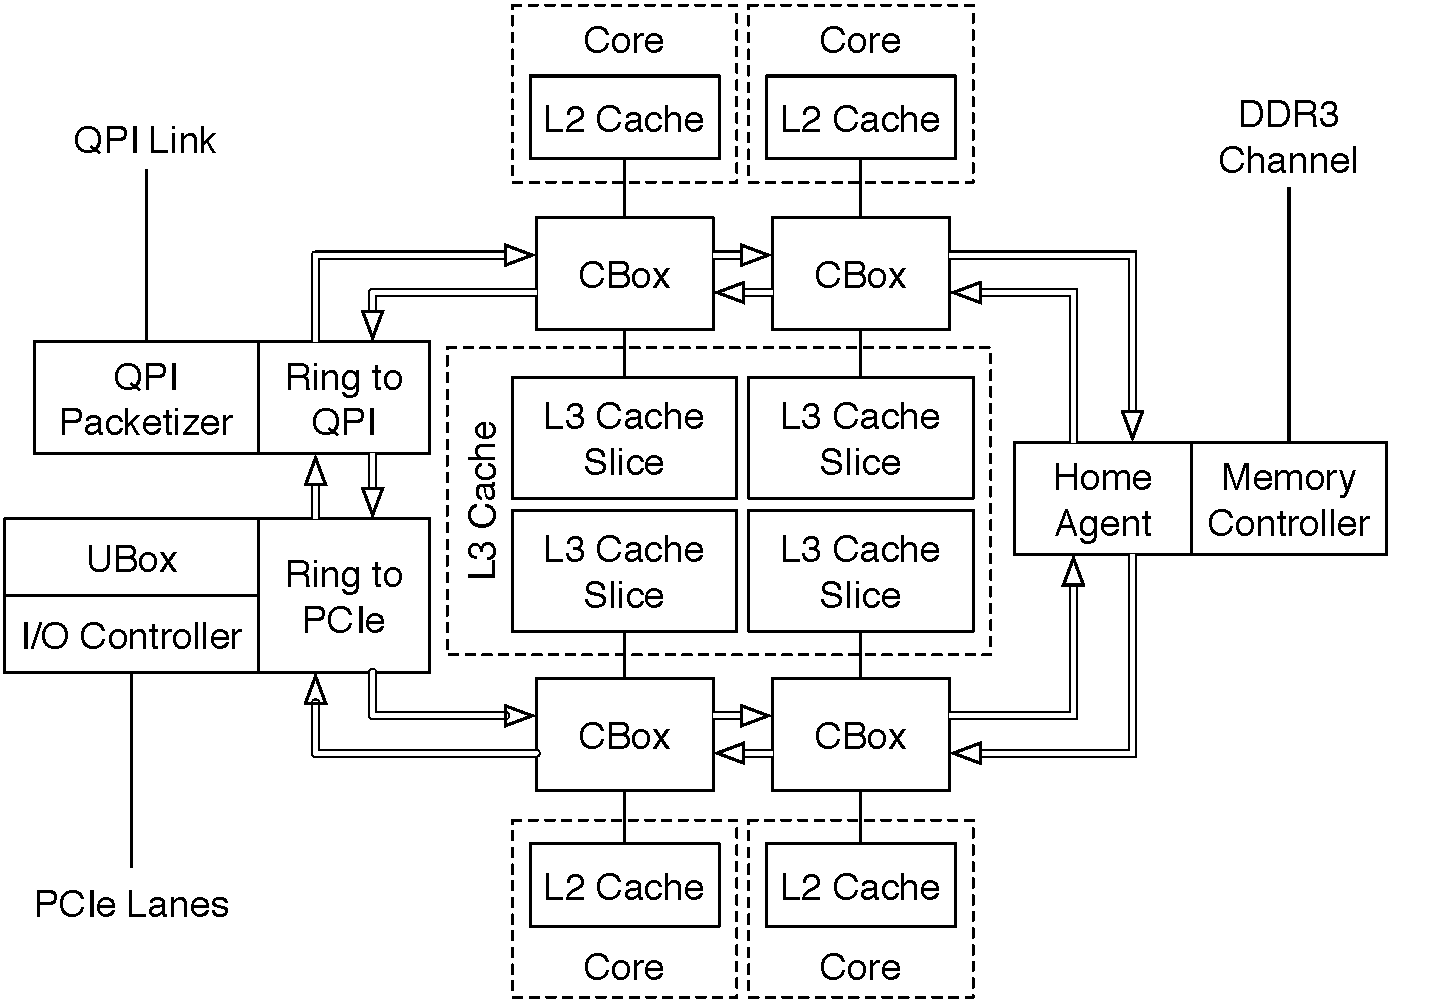
\includegraphics[width=90mm]{figures/cpu_uncore.pdf}
  \caption{
    The stops on the ring interconnect used for inter-core and core-uncore
    communication.
  }
  \label{fig:cpu_uncore}
\end{figure}

The number of LLC slices matches the number of cores in the CPU, and each LLC
slice shares a CBox with a core. The CBoxes implement the cache coherence
engine, so each CBox acts as the QPI cache agent for its LLC slice. CBoxes
use a \textit{Source Address Decoder} (SAD) to route DRAM requests to the
appropriate home agents. Conceptually, the SAD takes in a memory address and
access type, and outputs a transaction type (coherent, non-coherent, IO) and a
node ID. Each CBox contains a SAD replica, and the configurations of all SADs
in a package are identical.

The SAD configurations are kept in sync by the \textit{UBox}, which is the
uncore configuration controller, and connects the \textit{System agent} to the
ring. The UBox is responsible for reading and writing physically distributed
registers across the uncore. The UBox also receives interrupts from system and
dispatches them to the appropriate core.

On recent Intel processors, the uncore also contains at least one memory
controller. Each integrated memory controller (iMC or MBox in Intel's
documentation) is connected to the ring by a \textit{home agent} (HA or
\textit{BBox} in Intel's datasheets). Each home agent contains a
\textit{Target Address Decoder} (TAD), which maps each physical DRAM address to
a specific DRAM channel.

The integration of the memory controller on the CPU brings the ability to
filter DMA transfers. Accesses from a peripheral connected to the PCIe bus will
be handled by the integrated I/O controller (IIO) and placed on the ring
interconnect via the Ubox, then reach the iMC. Therefore, on modern systems,
DMA transfers go through both the SAD and TAD. Intel TXT takes advantage of
this to set up a protected DRAM range. For example, \cite{intel2015datasheet}
documents an ``Intel TXT DMA Protected Range'' IIO configuration register.
According to Intel's patents, the SGX implementation uses the same mechanism to
protect enclave memory from outside accesses.

Very recent processors also include the Generic Debug eXternal Connection
(GDXC) \cite{yuffe2011sandybridge, intel2011gdxc}, which collects and filters
ring traffic, and reports it to an external debugger. While GDXC is very useful
for debugging the CPU as well as the systems embedding it, it may compromise
the security of SGX enclaves. Due to the insufficient documentation on this
topic, this paper ignores the possibility of GDXC-based attacks. Fortunately,
a recent Intel patent \cite{shanbhogue2015gdxcsgx} indicates that Intel
engineers are tackling at least some classes of debugging bus attacks.
